\chapter{Le développement embryonnaire des vertébrés}\label{ch:b2:vertebrate-development}

Un œuf de grenouille est une sphère de deux millimètres de diamètre,
sombre en haut et pâle en bas. En une journée, il s'est divisé en
milliers de cellules~; en deux, un feuillet de ces cellules s'est
enroulé vers l'intérieur à travers un sillon pour former un intestin et
disposer une baguette le long du dos~; en trois, le feuillet situé
au-dessus de la baguette s'est replié en un tube qui deviendra
l'encéphale et la moelle épinière. Rien n'a été ajouté, sinon de l'eau.
L'information qui transforme une cellule en un têtard nageur était dans
l'œuf et dans son génome, et la manière dont elle se déploie ---
\omterm{def:b2:vertebrate-development:egg}{segmentation}, gastrulation, neurulation, \omterm{def:b2:vertebrate-development:induction}{induction} de chaque partie par
ses voisines --- est reconnaissable chez un poisson, un poulet et une
souris. Ce chapitre suit un embryon de vertébré à travers ces étapes et
décrit les expériences qui ont montré comment chacune de ses parties
apprend ce qu'elle doit devenir.

\section{De l'œuf à la blastula}

\begin{definition}[L'œuf et ses axes]\label{def:b2:vertebrate-development:egg}
\index{pole animal@pôle animal}\index{pole vegetatif@pôle végétatif}\index{vitellus}\index{segmentation}
Un œuf de vertébré est polarisé avant la fécondation~: le \emph{pôle
animal} contient le noyau et l'essentiel du cytoplasme, le \emph{pôle
végétatif} le \emph{vitellus}, la réserve de protéines et de lipides
dont l'embryon vivra jusqu'à ce qu'il se nourrisse. La quantité de
vitellus détermine tout ce qui suit~: un œuf d'oursin ou de mammifère
n'en contient presque pas et se segmente entièrement en cellules
égales~; un œuf de grenouille en contient une quantité moyenne et se
segmente entièrement mais inégalement (petites cellules en haut,
grosses cellules chargées de vitellus en bas)~; un œuf de poisson ou
d'oiseau est presque entièrement fait de vitellus et ne se segmente que
dans un disque de cytoplasme posé sur celui-ci. Chez la grenouille, le
point d'entrée du spermatozoïde fixe le second axe~: le cortex tourne de
trente degrés en s'en éloignant, découvrant un \emph{croissant gris} à
l'opposé du point d'entrée, et ce côté deviendra le dos. La
\emph{segmentation} est une série de mitoses rapides sans croissance ---
les cellules diminuent de moitié à chaque division --- pilotée par des
ARNm et des protéines maternels stockés dans l'œuf, les gènes propres
de l'embryon restant silencieux jusqu'à la \emph{transition
blastuléenne}, au bout d'une douzaine de divisions.
\end{definition}

\begin{omfigure}
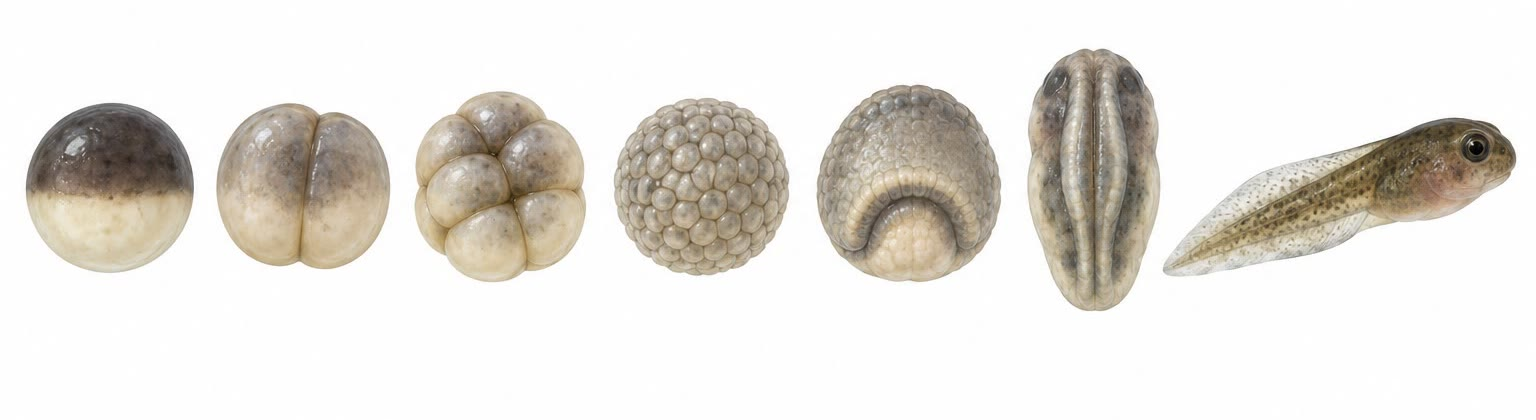
\includegraphics[width=0.9\linewidth]{images/book4/ai/b4-10-frog-development.jpg}

{\small Le développement d'une grenouille à partir de l'œuf fécondé~:
\omterm{def:b2:vertebrate-development:egg}{segmentation} jusqu'à la \omterm{def:b2:vertebrate-development:blastula}{blastula}, gastrulation, neurula avec ses
bourrelets neuraux, et têtard --- le tout en quelques jours, sans
croissance.}
\end{omfigure}

\begin{theorem}[L'arithmétique de la segmentation]\label{thm:b2:vertebrate-development:cleavage}
Après $k$ divisions synchrones, un œuf de volume $V_0$ forme $2^{k}$
cellules de volume moyen $V_0/2^{k}$ et de rayon $r_0/2^{k/3}$, et la
surface totale a été multipliée par $2^{k/3}$~; le rapport du volume
nucléaire au volume cytoplasmique, qui part d'environ $10^{-4}$ dans un
œuf de grenouille, est multiplié par $2^{k}$ et atteint celui d'une
cellule ordinaire ($\sim 0.1$) au bout d'une dizaine de divisions.
C'est ce rapport croissant --- le titrage d'un stock maternel fixe d'un
certain inhibiteur par une quantité d'ADN qui croît exponentiellement
--- qui déclenche la transition blastuléenne~: les divisions
ralentissent, deviennent asynchrones, et le génome zygotique s'active.
\end{theorem}
\begin{proof}
Le volume se conserve lors de la \omterm{def:b2:vertebrate-development:egg}{segmentation}~: chacune des $2^{k}$
cellules a donc un volume $V_0
2^{-k}$ et, en tant que sphère, un rayon $r_0 2^{-k/3}$~; leur surface
totale vaut
$2^{k}\cdot 4\pi r_0^{2}\, 2^{-2k/3} = 4\pi r_0^{2}\, 2^{k/3}$. Chaque
cellule garde un noyau de taille fixe, si bien que le rapport varie
comme $2^{k}$ à partir de $10^{-4}$~: $2^{10} = 1024$ le porte à $0.1$.
La transition de la grenouille se situe à la douzième division, ce qui
concorde avec un seuil atteint un peu plus tard.
\end{proof}
\begin{proof}[Faits expérimentaux]
Newport et Kirschner (1982) ajoutèrent de l'ADN supplémentaire à des
œufs de grenouille et constatèrent que la transition survenait plus tôt
d'autant de divisions que l'ADN était en excès~; retirer du cytoplasme
avait le même effet. L'horloge n'est ni le temps ni un compte de
divisions, mais un rapport.
\end{proof}

\begin{definition}[Blastula]\label{def:b2:vertebrate-development:blastula}
\index{blastula}\index{blastocoele@blastocœle}
La \omterm{def:b2:vertebrate-development:egg}{segmentation} aboutit à une \emph{blastula}~: une sphère creuse
(grenouille, oursin) ou un disque (poisson, oiseau) de quelques
milliers de cellules autour d'une cavité, le \emph{blastocœle}. Ses
cellules ont encore l'apparence de cellules non spécialisées, mais
elles ne sont pas équivalentes~: une \emph{carte des territoires
présomptifs}, établie en colorant des plages de la surface avec des
colorants vitaux et en les suivant, montre que la calotte animale
donnera la peau et le système nerveux (\emph{ectoderme}), la ceinture
équatoriale les muscles, le squelette, le rein et le sang
(\emph{mésoderme}), et la masse végétative l'intestin et ses organes
(\emph{endoderme}). Ces trois \emph{feuillets embryonnaires} sont les
mêmes chez tous les vertébrés, et l'étape suivante consiste à les mettre
en place~: le mésoderme et l'endoderme sont à l'extérieur et doivent
passer à l'intérieur.
\end{definition}

\section{Gastrulation et neurulation}

\begin{proposition}[La gastrulation]\label{prop:b2:vertebrate-development:gastrulation}
\index{gastrulation}\index{blastopore}\index{archenteron@archentéron}\index{notocorde}
La \emph{gastrulation} est l'ensemble des mouvements cellulaires qui
transforme la \omterm{def:b2:vertebrate-development:blastula}{blastula} à un seul feuillet en une \emph{gastrula} à trois
feuillets. Chez la grenouille, elle commence sous le croissant gris~:
les cellules y changent de forme en contractant leur extrémité externe
en bouteille, et la surface se creuse en un sillon, le
\emph{blastopore}. Par ce sillon, le mésoderme et l'endoderme
s'engouffrent vers l'intérieur (\emph{involution}), s'enroulant sur la
lèvre puis progressant le long du plafond de la cavité~; la calotte
animale s'étale vers le bas pour recouvrir l'extérieur
(\emph{épibolie})~; le blastopore se referme en un anneau autour des
dernières cellules chargées de \omterm{def:b2:vertebrate-development:egg}{vitellus}. À l'intérieur, une nouvelle
cavité bordée d'endoderme, l'\emph{archentéron}, est le futur intestin,
et le mésoderme entré le premier, le long de la ligne médiane, est
devenu une baguette rigide, la \emph{notocorde}, axe de tout embryon de
vertébré et structure qui donne son nom à l'embranchement. Chez les
oiseaux et les mammifères, les mêmes mouvements se font à travers une
fente, la \emph{ligne primitive}, dans un disque plat~; chez les
poissons, le disque s'étale sur le \omterm{def:b2:vertebrate-development:egg}{vitellus}. La chorégraphie diffère
selon le \omterm{def:b2:vertebrate-development:egg}{vitellus}~; le résultat --- ectoderme à l'extérieur, endoderme
bordant l'intestin, mésoderme entre les deux, notocorde sur la ligne
médiane --- est le même.
\end{proposition}

\begin{omfigure}
\begin{tikzpicture}[every node/.style={font=\scriptsize}, >=stealth]
  % blastula
  \begin{scope}
    \draw[thick, fill=omDef!15] (0,0) circle (1.3);
    \draw[thick, fill=white] (0,0.2) circle (0.75);
    \fill[omExo!40] (0,0) ++(-1.3,0) arc (180:360:1.3 and 1.3) -- cycle;
    \draw[thick] (0,0) circle (1.3);
    \node at (0,0.2) {blastocœle};
    \node[below, align=center] at (0,-1.45) {blastula\\calotte animale (en bleu), cellules à vitellus (en gris)};
  \end{scope}
  % early gastrula: blastopore forming
  \begin{scope}[xshift=4.2cm]
    \draw[thick, fill=omDef!15] (0,0) circle (1.3);
    \draw[thick, fill=white] (0,0.25) circle (0.7);
    \fill[omExo!40] (0,0) ++(-1.3,0) arc (180:360:1.3 and 1.3) -- cycle;
    \draw[thick] (0,0) circle (1.3);
    \draw[very thick, omThm] (1.0,-0.85) .. controls (0.5,-0.6) and (0.4,-0.3) .. (0.55,0.0);
    \draw[->, thick, omThm] (1.15,-0.7) .. controls (0.6,-0.4) .. (0.4,0.1);
    \draw[omThm] (1.0,-0.85) -- (0.9,-1.25); \node[omThm, anchor=north west] at (0.6,-1.2) {lèvre du blastopore};
    \node[below, align=center] at (0,-1.45) {jeune gastrula\\les cellules s'enroulent sur la lèvre};
  \end{scope}
  % late gastrula
  \begin{scope}[xshift=8.4cm]
    \draw[thick, fill=omDef!15] (0,0) circle (1.3);
    \draw[thick, fill=omExo!25] (0,0.05) circle (0.95);
    \draw[thick, fill=white] (0.15,-0.1) ellipse (0.55 and 0.4);
    \draw (0.6,-0.3) -- (1.6,-1.15); \node[anchor=west] at (1.6,-1.15) {archentéron};
    \draw[very thick, omThm] (-0.9,0.35) .. controls (-0.2,0.6) .. (0.8,0.4);
    \draw[omThm] (0.0,0.48) -- (-0.9,1.55); \node[omThm, anchor=east] at (-0.9,1.55) {notocorde};
    \draw[thick] (1.1,-0.7) -- (1.3,-0.5);
    \node[right] at (1.3,-0.5) {blastopore};
    \node[below, align=center] at (0,-1.45) {gastrula âgée~: trois feuillets,\\cavité intestinale, notocorde au plafond};
  \end{scope}
\end{tikzpicture}

{\small La gastrulation chez la grenouille, en coupe. Les cellules
s'enroulent vers l'intérieur sur la lèvre du blastopore~; l'endoderme
borde une nouvelle cavité intestinale, et le premier mésoderme à entrer
devient la notocorde le long de la ligne médiane.}
\end{omfigure}

\begin{proposition}[La neurulation et le plan d'organisation]\label{prop:b2:vertebrate-development:neurulation}
\index{neurulation}\index{tube neural}\index{somite}\index{crete neurale@crête neurale}
L'ectoderme situé au-dessus de la notocorde s'épaissit en une
\emph{plaque neurale}, dont les bords se soulèvent en bourrelets qui se
rejoignent sur la ligne médiane pour former le \emph{\omterm{prop:b2:vertebrate-development:neurulation}{tube neural}}, futur
encéphale et future moelle épinière, qui s'enfonce sous la peau~; des
cellules issues du sommet des bourrelets, la \emph{\omterm{prop:b2:vertebrate-development:neurulation}{crête neurale}},
migrent au loin pour former les nerfs périphériques, les cellules
pigmentaires, la médullosurrénale et une grande partie de la face. De
chaque côté de la notocorde, le mésoderme se segmente en blocs, les
\emph{somites}, une paire après l'autre de la tête vers la queue, qui
donnent les vertèbres, les muscles du tronc et le derme~; le mésoderme
latéral se clive en feuillets qui bordent la cavité générale et forment
le cœur et les membres~; le tube endodermique bourgeonne les poumons, le
foie et le pancréas. À la fin de la neurulation, l'embryon possède le
plan d'organisation des vertébrés --- un cordon nerveux dorsal au-dessus
d'une notocorde, un tube digestif ventral, une musculature segmentée,
une tête --- pour une longueur de quelques millimètres, et le reste du
développement consiste à élaborer les organes à partir de ce plan
(\cref{ch:b2:limb-organogenesis}).
\end{proposition}

\begin{omfigure}
\begin{tikzpicture}[every node/.style={font=\scriptsize}]
  \foreach \x/\lab in {0/{plaque neurale}, 4.0/{les bourrelets neuraux se soulèvent}, 8.0/{tube neural fermé~; migration de la crête neurale}} {
    \begin{scope}[xshift=\x cm]
      \draw[thick, fill=omExo!25] (-1.6,0) rectangle (1.6,-1.6);
      \draw[thick, omThm, fill=omThm!30] (0,-0.75) circle (0.28);
      \draw[thick, fill=omProp!30] (-1.3,-0.75) circle (0.32); \draw[thick, fill=omProp!30] (1.3,-0.75) circle (0.32);
      \node[below, align=center, text width=3.4cm] at (0,-1.7) {\lab};
    \end{scope}
  }
  \draw[very thick, omDef] (-1.6,0) -- (-0.7,0) .. controls (-0.3,0.15) and (0.3,0.15) .. (0.7,0) -- (1.6,0);
  \draw[very thick, omDef] (2.4,0) -- (3.3,0) .. controls (3.3,0.9) and (3.6,0.1) .. (4.0,0.0) .. controls (4.4,0.1) and (4.7,0.9) .. (4.7,0) -- (5.6,0);
  \draw[very thick, omDef] (6.4,0.05) -- (9.6,0.05);
  \draw[very thick, omDef, fill=omDef!20] (8.0,-0.3) circle (0.3);
  \foreach \p in {(7.35,-0.4),(8.65,-0.4)} \fill[omDef!70!black] \p circle (0.07);
  \node[omThm, anchor=west] at (9.8,-0.75) {notocorde};
  \node[omProp, anchor=west] at (9.8,-1.15) {somite};
  \node[omDef, anchor=west] at (9.8,-0.3) {tube neural};
  \node[omDef!70!black, anchor=west] at (9.8,0.1) {cellules de la crête neurale};
\end{tikzpicture}

{\small La neurulation en coupe transversale~: l'ectoderme situé
au-dessus de la notocorde (en rouge) s'épaissit, se replie et se ferme
en \omterm{prop:b2:vertebrate-development:neurulation}{tube neural} (en bleu), tandis que le mésoderme bordant la notocorde
se segmente en somites (en orange) et que des cellules de la \omterm{prop:b2:vertebrate-development:neurulation}{crête
neurale} quittent les bourrelets en train de se fermer.}
\end{omfigure}

\begin{omfigure}
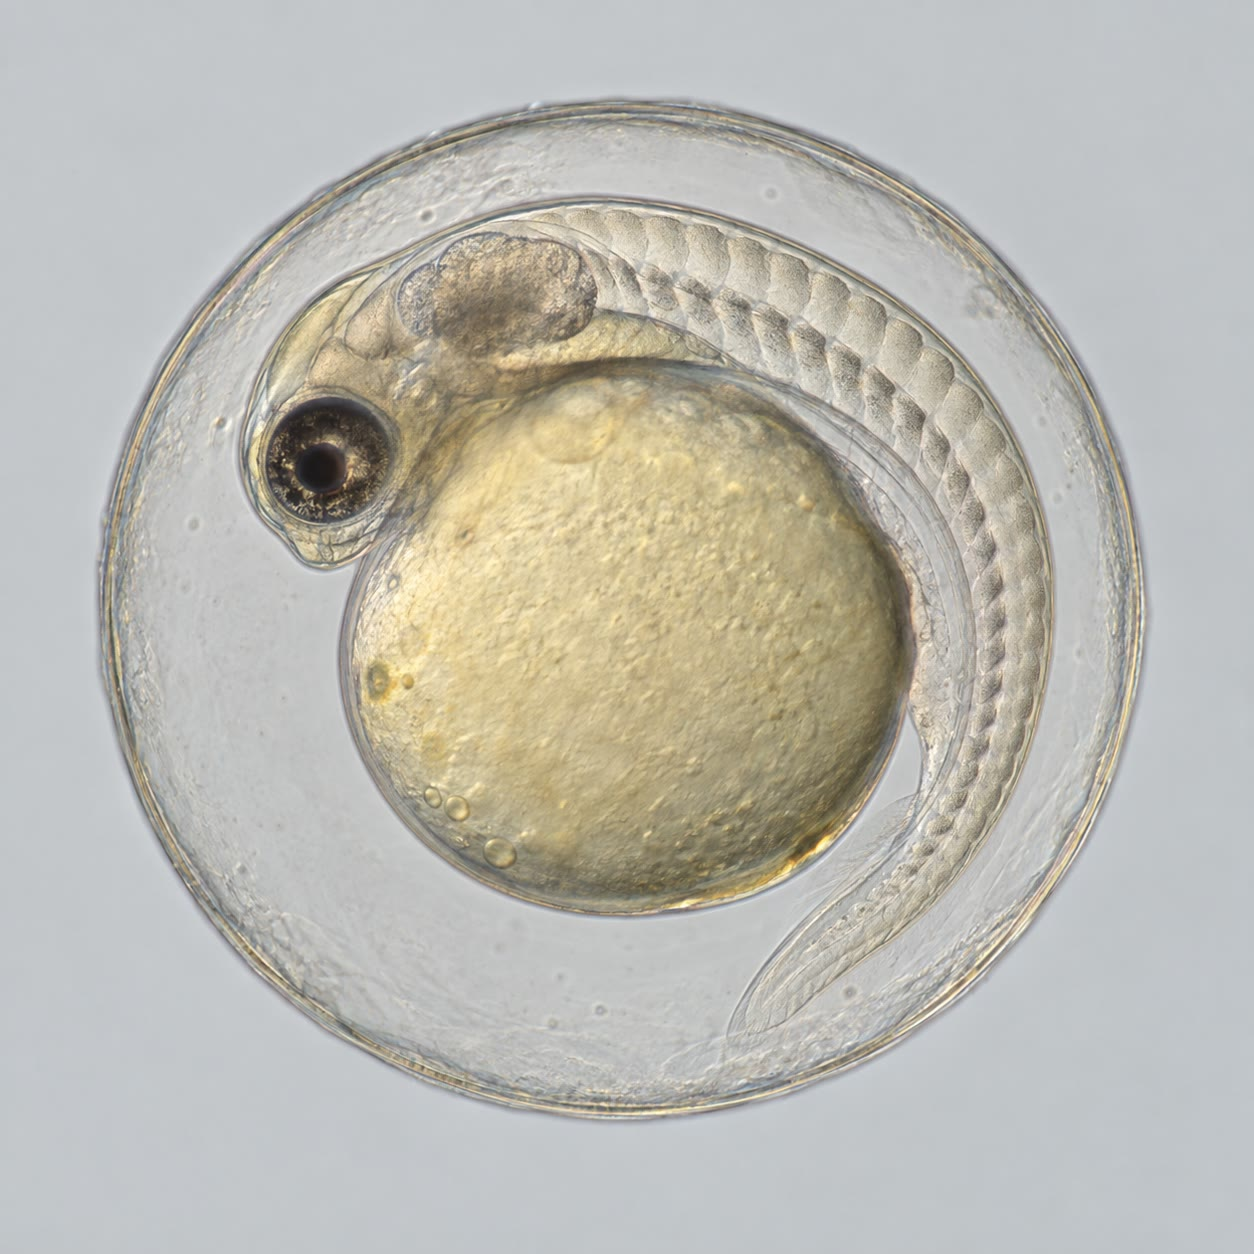
\includegraphics[width=0.42\linewidth]{images/book4/ai/b4-10-zebrafish-embryo.jpg}\hspace{0.04\linewidth}
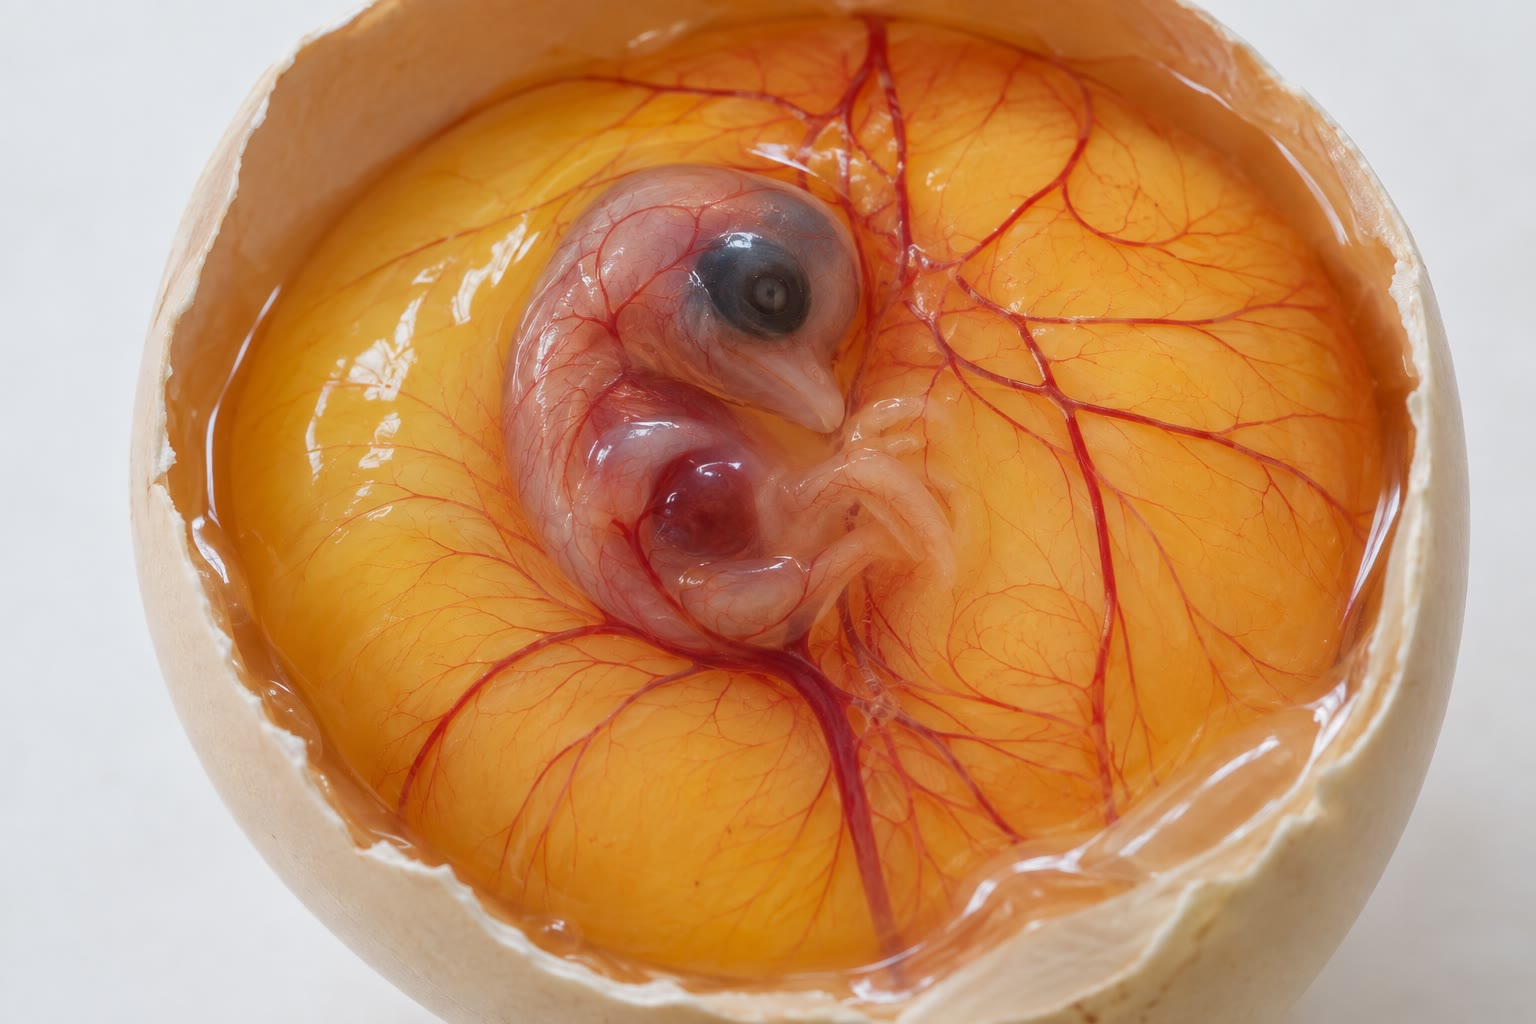
\includegraphics[width=0.5\linewidth]{images/book4/ai/b4-10-chick-embryo.jpg}

{\small À gauche~: un embryon de poisson zèbre âgé d'un jour dans son
chorion, enroulé autour de son \omterm{def:b2:vertebrate-development:egg}{vitellus}, avec l'œil, l'encéphale et une
rangée de somites. À droite~: un embryon de poulet de trois jours sur son
\omterm{def:b2:vertebrate-development:egg}{vitellus}, le cœur battant déjà et les vaisseaux s'étendant sur le
\omterm{def:b2:vertebrate-development:egg}{vitellus} pour le nourrir.}
\end{omfigure}

\section{L'induction~: comment les cellules apprennent où elles sont}

\begin{definition}[Induction et compétence]\label{def:b2:vertebrate-development:induction}
\index{induction (embryonnaire)}\index{competence@compétence}\index{organisateur}
L'\emph{induction} est le processus par lequel un groupe de cellules
modifie, par un signal, le destin d'un groupe voisin~; les cellules qui
répondent doivent être \emph{compétentes} --- capables de répondre, ce
qu'elles ne sont que pendant un temps limité. Le développement est une
chaîne d'inductions~: les cellules végétatives induisent le mésoderme
dans les cellules situées au-dessus d'elles~; le mésoderme dorsal ---
l'\emph{organisateur}, à la lèvre du blastopore --- induit la plaque
neurale dans l'ectoderme qui le surmonte et organise le mésoderme de
part et d'autre~; la notocorde induit le plancher du \omterm{prop:b2:vertebrate-development:neurulation}{tube neural}~; la
vésicule optique, un bourgeon de l'encéphale, induit un cristallin dans
la peau qu'elle touche~; le cristallin induit la cornée. Chaque tissu
induit devient l'inducteur du suivant. Les signaux appartiennent à une
poignée de familles de protéines sécrétées, utilisées encore et encore
--- les mêmes qui organisent un membre (\cref{ch:b2:limb-organogenesis})
et, chez l'adulte, assurent la signalisation du
\cref{ch:b2:cell-signalling}.
\end{definition}
\begin{proof}[Faits expérimentaux]
Spemann et Mangold (1924) prélevèrent la lèvre dorsale du blastopore
d'une jeune gastrula d'une espèce de triton et la greffèrent sur la face
ventrale d'une gastrula d'une autre espèce, de pigmentation différente,
afin de distinguer les cellules de l'hôte de celles du greffon. Le
greffon ne devint pas simplement ce qu'il serait devenu en place~: il
s'enroula vers l'intérieur, forma une notocorde et \emph{induisit
l'ectoderme ventral de l'hôte lui-même} à former un second \omterm{prop:b2:vertebrate-development:neurulation}{tube neural}
et, à côté de celui-ci, des somites de l'hôte --- un second embryon
complet, fait en grande partie de cellules de l'hôte, soudé ventre à
ventre au premier. Aucun autre fragment de la gastrula n'en était
capable. Ils appelèrent cette lèvre l'\omterm{def:b2:vertebrate-development:induction}{organisateur}~; ses signaux (des
protéines qui bloquent le facteur ventralisant BMP) furent identifiés
soixante-dix ans plus tard.
\end{proof}

\begin{omfigure}
\begin{tikzpicture}[every node/.style={font=\scriptsize}, >=stealth]
  % donor
  \draw[thick, fill=omDef!12] (0,0) circle (1.3); \node[above] at (0,1.4) {gastrula donneuse (pâle)};
  \draw[very thick, omThm] (0.85,-0.95) arc (-45:-20:1.3); \node[omThm, right] at (1.2,-0.8) {lèvre dorsale};
  \draw[->, thick] (1.6,-0.3) -- (3.4,-0.3);
  % host
  \draw[thick, fill=omExo!45] (5,0) circle (1.3); \node[above] at (5,1.4) {gastrula hôte (sombre)};
  \draw[very thick, omThm] (5.85,-0.95) arc (-45:-20:1.3); \node[omThm, right] at (6.2,-0.8) {propre lèvre};
  \draw[very thick, omThm] (4.15,0.95) arc (135:160:1.3); \node[omThm, left] at (3.9,1.0) {greffon};
  \draw[->, thick] (6.6,-0.3) -- (8.4,-0.3);
  % result: twinned embryo
  \draw[thick, fill=omExo!45] (10.6,0) ellipse (1.8 and 1.1);
  \draw[very thick, omDef!70!black] (9.2,0.5) .. controls (10.0,0.8) and (11.2,0.8) .. (12.0,0.5);
  \draw[very thick, omDef!70!black] (9.2,-0.5) .. controls (10.0,-0.8) and (11.2,-0.8) .. (12.0,-0.5);
  \node[above] at (10.6,1.2) {résultat~: deux axes};
  \node[anchor=north, align=center, text width=4cm] at (10.6,-1.2) {un second tube neural et des somites, faits de cellules \emph{de l'hôte}, induits par le greffon};
\end{tikzpicture}

{\small L'expérience de l'\omterm{def:b2:vertebrate-development:induction}{organisateur}. Une lèvre dorsale greffée sur le
ventre d'une autre gastrula induit les cellules de l'hôte à former un
second axe embryonnaire.}
\end{omfigure}

\begin{theorem}[Un gradient de morphogène]\label{thm:b2:vertebrate-development:gradient}
\index{morphogene@morphogène}
De nombreuses \omterm{def:b2:vertebrate-development:induction}{inductions} passent par un \emph{morphogène}~: un signal
sécrété par une source, qui se répand dans le tissu et que les cellules
lisent selon sa concentration locale --- au-dessus d'un seuil un destin,
au-dessus d'un seuil plus élevé un autre. Un morphogène produit par une
source plane à un débit $j$ par unité de surface, diffusant avec un
coefficient $D$ et dégradé avec une constante de vitesse $k$, a en
régime stationnaire le profil exponentiel
\[
c(x) = c_0\,e^{-x/\lambda}, \qquad \lambda = \sqrt{D/k}, \qquad c_0 = \frac{j}{\sqrt{Dk}},
\]
de sorte que la distance à laquelle la concentration passe sous un
seuil $T$ vaut $x_T = \lambda\ln(c_0/T)$~: un tissu peut être découpé en
bandes de largeur fixe par des seuils fixes. Avec $D =
\qty{1e-12}{m^2/s}$ (une protéine ralentie par les liaisons qu'elle
contracte en traversant le tissu) et $k = \qty{1e-3}{s^{-1}}$ (une
demi-vie d'environ douze minutes), $\lambda = \sqrt{10^{-9}}\,\unit{m} \approx
\qty{32}{\micro m}$~: quelques diamètres cellulaires,
l'échelle à laquelle s'organisent les champs embryonnaires. Doubler la
source double $c_0$ et déplace chaque frontière vers l'extérieur de $\lambda
\ln 2$.
\end{theorem}
\begin{proof}
En régime stationnaire, la diffusion équilibre la dégradation~:
$D\,c'' = k\,c$, dont la solution décroissante est
$c = c_0 e^{-x/\lambda}$ avec $\lambda^2 =
D/k$. Le flux qui quitte la source vaut $-Dc'(0) = Dc_0/\lambda = j$,
ce qui donne $c_0 = j\lambda/D = j/\sqrt{Dk}$. Poser $c(x_T) = T$ donne
$x_T$~; remplacer $c_0$ par $2c_0$ lui ajoute $\lambda\ln 2$.
\end{proof}

\begin{omfigure}
\begin{tikzpicture}
\begin{axis}[
  width=0.78\linewidth, height=5.6cm,
  axis x line=bottom, axis y line=left,
  xmin=0, xmax=120, ymin=0, ymax=1.1,
  xlabel={distance à la source (\unit{\micro m})}, ylabel={morphogène (relatif)},
  xlabel style={font=\small, at={(axis description cs:0.5,-0.13)}, anchor=north},
  ylabel style={font=\small},
  tick label style={font=\small}, xtick={0,32,64,96}, ytick={0,0.5,1},
  clip=false,
]
\fill[omThm!18] (axis cs:0,0) rectangle (axis cs:22,1.05); \node[font=\scriptsize, anchor=south] at (axis cs:11,1.05) {destin A};
\fill[omProp!18] (axis cs:22,0) rectangle (axis cs:61,1.05); \node[font=\scriptsize, anchor=south] at (axis cs:41,1.05) {destin B};
\fill[omExo!18] (axis cs:61,0) rectangle (axis cs:120,1.05); \node[font=\scriptsize, anchor=south] at (axis cs:90,1.05) {destin C};
\addplot[very thick, omDef, domain=0:120, samples=80] {exp(-x/32)};
\draw[dashed, gray] (axis cs:0,0.5) -- (axis cs:22,0.5) -- (axis cs:22,0);
\draw[dashed, gray] (axis cs:0,0.15) -- (axis cs:61,0.15) -- (axis cs:61,0);
\node[font=\scriptsize, anchor=west] at (axis cs:62,0.55) {seuil 1};
\node[font=\scriptsize, anchor=west] at (axis cs:62,0.2) {seuil 2};
\end{axis}
\end{tikzpicture}

{\small Un gradient de morphogène avec $\lambda = \qty{32}{\micro m}$.
Deux seuils découpent le tissu en trois bandes de destins cellulaires
dont les largeurs sont fixées par $\lambda$ et par les rapports des
seuils à la concentration de la source.}
\end{omfigure}

\begin{example}[Lire le gradient]\label{ex:b2:vertebrate-development:reading}
Dans la gastrula de grenouille, les cellules de la zone marginale
exposées à des quantités graduées d'un signal de la famille de
l'activine deviennent, de la dose la plus forte à la plus faible,
notocorde, muscle, rein et sang~; des cellules dissociées de calotte
animale placées dans une boîte avec une dose proche d'un seuil changent
de destin pour un facteur deux de concentration. Dans le \omterm{prop:b2:vertebrate-development:neurulation}{tube neural},
un signal issu de la notocorde et de la plaque du plancher se répand
vers le haut et spécifie, en partant du bas, les motoneurones puis des
classes successives d'interneurones, à des seuils distants de quelques
diamètres cellulaires. Les coordonnées de l'organisme sont écrites en
concentrations.
\end{example}

\section{Destin, engagement et calendrier des décisions}

\begin{proposition}[Quand le destin d'une cellule est fixé]\label{prop:b2:vertebrate-development:commitment}
\index{determination@détermination}\index{regulation (embryonnaire)@régulation (embryonnaire)}
Le \emph{destin} d'une cellule est ce qu'elle deviendra normalement~; sa
\emph{potentialité} est ce qu'elle peut devenir si on la déplace~; elle
est \emph{déterminée} lorsque son destin ne change plus avec son
environnement. Les jeunes embryons sont \emph{régulateurs}~: chacun des
deux premiers blastomères de grenouille, séparés, forme un petit têtard
entier, et les premières cellules d'un embryon de mammifère sont toutes
totipotentes --- c'est ainsi que naissent les vrais jumeaux. La
détermination s'installe progressivement et à des moments différents
selon les tissus~: un fragment d'ectoderme de jeune gastrula greffé sur
le ventre devient de la peau ventrale, alors que le même fragment
prélevé sur une gastrula âgée forme une plaque neurale où qu'on le
place~; au stade du bourgeon caudal, un champ de membre transplanté sur
le flanc y forme un membre. Chez la plupart des invertébrés, au
contraire, le destin est fixé tôt par le cytoplasme dont hérite chaque
cellule (développement \emph{en mosaïque}), et un blastomère séparé ne
forme que sa partie. La stratégie des vertébrés --- garder les cellules
flexibles et leur dire quoi faire par \omterm{def:b2:vertebrate-development:induction}{induction} --- est ce qui rend
possibles la gémellité, la régénération et l'expérience de
l'\omterm{def:b2:vertebrate-development:induction}{organisateur}.
\end{proposition}
\begin{proof}[Faits expérimentaux]
Spemann (1901) serra une boucle de cheveu autour d'un œuf de triton au
stade deux cellules~: si la boucle se trouvait dans le plan du croissant
gris, de sorte que chaque moitié en recevait une partie, deux embryons
complets se formaient~; si elle lui était perpendiculaire, de sorte
qu'une moitié recevait tout le croissant, cette moitié formait un
embryon et l'autre une boule de tissu ventral. Le croissant --- le futur
\omterm{def:b2:vertebrate-development:induction}{organisateur} --- était la seule partie qui ne pouvait pas être divisée.
\end{proof}

\begin{example}[Le calendrier d'une grenouille]\label{ex:b2:vertebrate-development:timetable}
À \qty{18}{\celsius}~: fécondation~; première division à \qty{1.5}{h},
puis toutes les demi-heures~; \omterm{def:b2:vertebrate-development:blastula}{blastula} de \num{4000} cellules à
\qty{7}{h}~; transition blastuléenne à \qty{8}{h}~; gastrulation de
\qty{10}{h} à \qty{20}{h}~; fermeture des bourrelets neuraux à
\qty{30}{h}~; battements cardiaques à \qty{2.5}{d}~; éclosion et début
de l'alimentation à \qty{4}{d}, sous forme d'un têtard de \qty{6}{mm}.
Un poisson zèbre fait de même en un jour, un poulet en trois, une
souris en neuf~; un embryon humain gastrule au cours de la troisième
semaine et ferme son \omterm{prop:b2:vertebrate-development:neurulation}{tube neural} avant la fin de la quatrième --- avant
que la plupart des femmes ne sachent qu'elles sont enceintes, et c'est
pourquoi l'acide folique, nécessaire à la fermeture du \omterm{prop:b2:vertebrate-development:neurulation}{tube neural}, est
prescrit avant la conception.
\end{example}

\section{Exercices}

\begin{exercise}[$\star$]\label{exo:b2:vertebrate-development:1}
Définir \omterm{def:b2:vertebrate-development:egg}{segmentation}, \omterm{def:b2:vertebrate-development:blastula}{blastula}, gastrulation et neurulation, et nommer
la structure que produit chaque étape.
\end{exercise}

\begin{exercise}[$\star$]\label{exo:b2:vertebrate-development:2}
Donner les trois feuillets embryonnaires et, pour chacun, quatre tissus
adultes qui en dérivent.
\end{exercise}

\begin{exercise}[$\star$]\label{exo:b2:vertebrate-development:3}
Comment la quantité de \omterm{def:b2:vertebrate-development:egg}{vitellus} modifie-t-elle le mode de \omterm{def:b2:vertebrate-development:egg}{segmentation}
et de gastrulation~? Comparer une grenouille et un poulet.
\end{exercise}

\begin{exercise}[$\star$]\label{exo:b2:vertebrate-development:4}
Qu'est-ce que l'\omterm{def:b2:vertebrate-development:induction}{induction}~? Donner trois \omterm{def:b2:vertebrate-development:induction}{inductions} dans l'ordre où elles
se produisent dans un embryon de grenouille, en nommant l'inducteur et
le tissu qui répond.
\end{exercise}

\begin{exercise}[$\star\star$]\label{exo:b2:vertebrate-development:5}
Un œuf de grenouille de rayon \qty{1}{mm} subit douze divisions.
Calculer le nombre de cellules, leur rayon moyen, et le facteur par
lequel la surface cellulaire totale a été multipliée. Pourquoi l'embryon
a-t-il besoin de cette surface supplémentaire~?
\end{exercise}

\begin{exercise}[$\star\star$]\label{exo:b2:vertebrate-development:6}
Le rapport nucléocytoplasmique part de $10^{-4}$, et la transition
blastuléenne survient lorsqu'il atteint $0.4$. Au bout de combien de
divisions~? Si l'on injecte dans l'œuf trois fois sa propre quantité
d'ADN, à quelle division la transition survient-elle~?
\end{exercise}

\begin{exercise}[$\star\star$]\label{exo:b2:vertebrate-development:7}
Un morphogène a $D = \qty{2e-12}{m^2/s}$ et une demi-vie de
\qty{10}{min}. Calculer $k$ et $\lambda$. Deux seuils se situent à
\qty{50}{\%} et à \qty{10}{\%} de la concentration de la source~: donner
les largeurs des trois bandes de destins.
\end{exercise}

\begin{exercise}[$\star\star$]\label{exo:b2:vertebrate-development:8}
Dans le gradient de l'exercice précédent, une \omterm{def:b2:genome-diversification:mutation}{mutation} double la
source. De combien chaque frontière se déplace-t-elle~? Et si c'est la
constante de dégradation qui double~?
\end{exercise}

\begin{exercise}[$\star\star$]\label{exo:b2:vertebrate-development:9}
Décrire l'expérience de Spemann et Mangold, dire pourquoi les deux
espèces devaient différer par leur pigmentation, et indiquer ce que le
résultat a exclu.
\end{exercise}

\begin{exercise}[$\star\star\star$]\label{exo:b2:vertebrate-development:10}
Prévoir le résultat~: (a) d'un fragment de plaque neurale présomptive de
jeune gastrula greffé sur le ventre~; (b) du même fragment prélevé sur
une gastrula âgée~; (c) d'un fragment d'ectoderme ventral placé
au-dessus d'une notocorde dans une gastrula âgée~; (d) de l'ablation de
tout l'\omterm{def:b2:vertebrate-development:induction}{organisateur} d'une jeune gastrula. Expliquer chaque cas à l'aide
des notions de \omterm{def:b2:vertebrate-development:induction}{compétence} et de détermination.
\end{exercise}

\begin{exercise}[$\star\star\star$]\label{exo:b2:vertebrate-development:11}
La première division de la grenouille dure \qty{90}{min} et les onze
suivantes \qty{30}{min} chacune, à \qty{18}{\celsius}~; à
\qty{10}{\celsius}, chaque étape est 2.5 fois plus lente. À quel moment
la transition blastuléenne est-elle atteinte à chaque température~?
Expliquer pourquoi la transition survient au même nombre de cellules aux
deux températures, et ce que cela indique sur l'horloge.
\end{exercise}

\begin{exercise}[$\star\star\star$]\label{exo:b2:vertebrate-development:12}
«~Un embryon de vertébré se construit par la conversation, un embryon
d'invertébré par l'héritage.~» Discuter le contraste entre développement
régulateur et développement en mosaïque, ses conséquences pour la
gémellité et la régénération, et pourquoi il s'agit d'une différence de
degré.
\end{exercise}

\section{Problème~: un embryon de grenouille chronométré et organisé}

\begin{problem}[{Problème du week-end --- un embryon de grenouille suivi à
travers la segmentation, la transition blastuléenne, la gastrulation et
l'induction, avec le calcul du gradient de morphogène et la prévision
des greffes classiques, jusqu'au nombre de cellules et au moment de la
transition et aux largeurs des bandes de destins}]
\label{pb:b2:vertebrate-development:1}
Un œuf de grenouille a un rayon de \qty{0.7}{mm} et un noyau de rayon
\qty{0.03}{mm} dont le contenu en ADN vaut $c$~; chaque division dure
\qty{30}{min}, après une première de \qty{75}{min}. La transition
blastuléenne survient lorsque l'ADN total atteint $4000\,c$.
Morphogène~: $D =
\qty{1e-12}{m^2/s}$, demi-vie \qty{20}{min}, concentration à la source
$c_0$, seuils à $0.4\,c_0$ et $0.08\,c_0$.

\medskip
\noindent\textbf{Partie I --- La \omterm{def:b2:vertebrate-development:egg}{segmentation}.}
\begin{enumerate}
  \item Calculer le volume de l'œuf et celui de son noyau, et le rapport
        nucléocytoplasmique initial.
  \item Au bout de combien de divisions l'ADN atteint-il $4000\,c$~?
        Combien de cellules~?
  \item À quel moment après la fécondation~?
  \item Quel est alors le rayon cellulaire moyen, et le rapport du volume
        nucléaire au volume cellulaire si les noyaux gardent leur
        taille~? Commenter.
  \item Par quel facteur la surface cellulaire totale a-t-elle été
        multipliée~?
  \item Chaque division exige la copie du génome~: quelle quantité d'ADN
        a été synthétisée au total, en unités de $c$, et pourquoi
        l'embryon n'a-t-il pas besoin de transcrire ses gènes pour
        cela~?
  \item Qu'est-ce qui change à la transition, et quelle expérience
        montre qu'elle est déclenchée par un rapport et non par un
        compte~?
\end{enumerate}

\medskip
\noindent\textbf{Partie II --- La gastrulation.}
\begin{enumerate}[resume]
  \item Où le blastopore se forme-t-il par rapport au point d'entrée du
        spermatozoïde, et qu'est-ce qui a fixé cette position~?
  \item Énumérer, dans l'ordre, les tissus qui s'enroulent à travers le
        blastopore et leur position ensuite.
  \item La gastrulation dure \qty{10}{h} et le feuillet qui s'enroule
        parcourt \qty{2}{mm}. Calculer la vitesse moyenne des cellules en
        micromètres par minute et la comparer à celle d'un fibroblaste
        qui rampe (\qty{1}{\micro m/min}).
  \item Pourquoi la gastrulation est-elle impossible avant la transition
        blastuléenne~?
  \item Expliquer en une phrase pourquoi c'est la notocorde, et non le
        \omterm{prop:b2:vertebrate-development:neurulation}{tube neural}, qui est la structure caractéristique des cordés.
  \item Un médicament qui bloque les changements de forme des cellules
        est appliqué au début de la gastrulation. Prévoir l'embryon.
\end{enumerate}

\medskip
\noindent\textbf{Partie III --- Le gradient.}
\begin{enumerate}[resume]
  \item Calculer $k$ à partir de la demi-vie, puis $\lambda$.
  \item Calculer les positions des deux seuils.
  \item Donner les largeurs des trois bandes de destins en micromètres
        et en cellules de \qty{15}{\micro m}.
  \item La source est divisée par deux. Recalculer les deux positions et
        indiquer quelle bande rétrécit le plus.
  \item Une cellule située à \qty{60}{\micro m} de la source est
        déplacée à \qty{10}{\micro m} avant la lecture du gradient~; puis
        après. Que devient-elle dans chaque cas, et pourquoi~?
  \item Expliquer pourquoi un profil exponentiel donne des frontières
        dont la position dépend du logarithme de l'intensité de la
        source, et pourquoi cela rend l'organisation robuste.
\end{enumerate}

\medskip
\noindent\textbf{Partie IV --- Les greffes.}
\begin{enumerate}[resume]
  \item Prévoir le résultat de la greffe d'une lèvre dorsale sur la face
        ventrale d'une jeune gastrula, et celui de la greffe de zone
        marginale ventrale sur la face dorsale.
  \item Prévoir le résultat de la greffe d'une lèvre dorsale sur la face
        ventrale d'une \emph{neurula}, et expliquer la différence.
  \item Un embryon de grenouille au stade deux cellules est séparé dans
        le plan du croissant gris~; un autre perpendiculairement à ce
        plan. Prévoir les deux résultats.
  \item Une calotte animale est prélevée sur une \omterm{def:b2:vertebrate-development:blastula}{blastula} et cultivée
        seule~; la même calotte est cultivée au contact de cellules
        végétatives. Prévoir les tissus formés.
  \item Pourquoi le résultat de Spemann et Mangold exigeait-il que l'hôte
        et le greffon soient distinguables, et qu'aurait pu montrer une
        greffe entre espèces différentes~?
  \item Énoncer le résultat~: le numéro de la division et le moment de
        la transition, le nombre de cellules correspondant, et les trois
        largeurs de bandes.
\end{enumerate}
\end{problem}
